\documentclass[12pt,a4paper]{scrreprt}
\usepackage[latin1]{inputenc}
\usepackage{amsmath}
\usepackage{amsfonts}
\usepackage{amssymb}
\usepackage{pgf}
\usepackage{graphics, gincltex}
\usepackage{hyperref}
\usepackage{color}
\hypersetup{colorlinks=true}

\newcommand{\karbon}{\texttt{KARBON {}}}
\newcommand{\HRule}{\rule{\linewidth}{0.5mm}}

\author{Ioannis Charalampidis}
\title{KARBON User's Guide}

\begin{document}

\begin{titlepage}
\begin{center}
	% Upper part of the page
	
\includegraphics[width=0.4\textwidth]{cernlogo.pdf}\\[1cm]    

	\textsc{\LARGE PH-SFT Group}\\[1.5cm]
	\textsc{\Large Application performance testing for CernVM}\\[0.5cm]

	% Title
	\HRule \\[0.4cm] { 
		\huge \bfseries KARBON Application Profiler
		}\\[0.4cm]
	\HRule \\[0.4cm]
	
	\textsc{Version 0.4 beta}\\[1.5cm]

	% Author and supervisor
	\begin{minipage}{0.4\textwidth}
		\begin{flushleft} 
			\large\emph{Author:}\\
			Ioannis \textsc{Charalampidis}
		\end{flushleft}
	\end{minipage}
	\begin{minipage}{0.4\textwidth}
		\begin{flushright} \large
			\emph{Supervisor:} \\
			Predrag \textsc{Buncic}
		\end{flushright}
	\end{minipage}

	\vfill

	% Bottom of the page
	{\large \today}
\end{center}
\end{titlepage}


\tableofcontents
\newpage

\chapter{Overview}

\karbon is a platform-independent visual application profiling tool written in Java, based on system call tracing. It processes trace files generated by strace, systemTAP or similar call tracing applications and displays the application performance results in a user-friendly graphical interface (Figure \ref{screen}). It is capable of tracking network I/O, disk I/O and core OS operations, such as process management and signalling. Keep in mind that this application can not track memory access since it is not implemented through system calls. However memory access implemented using the mmap() is tracked.

\begin{figure}
	\centering
    	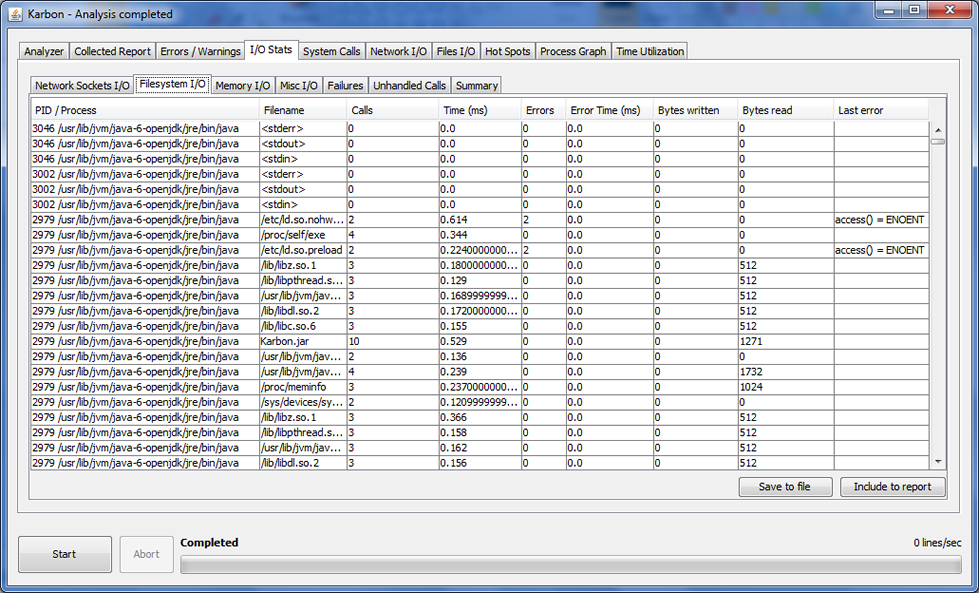
\includegraphics[]{screen-14.png}
	\caption{The \karbon User interface after the trace file analysis}
	\label{screen}
\end{figure}

\karbon has a modular design and a simple API that allows anyone to extend it's functionality. With the currently developed extensions, \karbon is capable of performing the following tasks:
\begin{itemize}
	\item Collect statistics regarding system calls, such as: number of hits on each system call, mostly used system calls, failures, time penalties, "hot" spots etc.
	\item Track the evolution of file descriptors though time and group accordingly all the relevant system calls.
	\item Map the file descriptors to file names, network sockets or memory mappings and display the usage of the relevant system calls.
	\item Track the lifespan of child processes on multi-threaded applications and generate relation graphs.
	\item Display collective information that help detect bottlenecks and time-consuming operations.
\end{itemize}

After the trace file is analysed, it is possible to generate custom reports that can be exported for further processing or presentation.

\chapter{Getting Started}
\section{Requirements}
In order to run \karbon you need to have Java Runtime 6.0 or later installed on your machine. You can get the latest available version from the official website\footnote{You can find the latest Java releases here: \url{http://www.oracle.com/technetwork/java/javase/downloads/index.html}}.

You also need a system call tracing application in order to generate a trace file. It's recommended to use the latest version of {\tt strace}\footnote{You can get the latest version of STrace from here: \url{http://sourceforge.net/projects/strace/}}.

Additionally, if you want to perform a real-time analysis from a remote machine you need a socket client that reads from STDIN such as {\tt netcat}.

\section{Usage}
There are mainly two ways to use \karbon:
\begin{enumerate}
	\item Trace the application independantly, generate the trace file and then pass it to \karbon for analysis.
	\item Run an application and perform real-time analysis with \karbon \textit{(Experimental)}.
\end{enumerate}

\subsection{Example of separated tracing/analysis setup}
In this case, you have to generate the trace log manually and then pass the output file to \karbon for analysis. To do so, you need to do the following:
\begin{enumerate}
	\item Install {\tt strace} on the machine you want to perform the trace onto.
	\item Run your application under tracer using the following command:\\[0.2cm]
		{\tt strace -Ttttf -s 128 -o <tracefile> -- <application> <arguments>}
	\item Copy the trace file to the machine that will run \karbon
	\item Start \karbon by double-clicking the .jar file, using the start.sh or start.bat, or by invoking the following command:\\[0.2cm]
		{\tt java -jar Karbon.jar}
	\item On the Analyzer tab select the \textbf{From file} tab
	\item Click \textbf{Browse} and select the trace file
	\item Load the required plug-ins by checking the check-boxes in the list or click \textbf{All} to load them all. \textit{(Keep in mind that there are dependencies between plugins and some of them will be loaded automatically even if you don't select them.)}
	\item Click \textbf{Start}
\end{enumerate}

\subsection{Example of real-time analysis setup}
\karbon supports TCP and UDP streaming input, allowing it to receive real-time logs from a remote machine without a need of an intermediate log file. To do so, you need to do the following:
\begin{enumerate}
	\item Install {\tt strace} and {\tt netcat} on the machine you want to perform the trace onto.
	\item Start \karbon by double-clicking the .jar file, using the start.sh or start.bat, or by invoking the following command:\\[0.2cm]
		{\tt java -jar Karbon.jar}
	\item Select the \textbf{From TCP Stream} tab. You can change the port number but it is recommended to leave the port number to 1225. 
	\item Load the required plug-ins by checking the check-boxes in the list or click \textbf{All} to load them all. \textit{(Keep in mind that there are dependencies between plugins and some of them will be loaded automatically even if you don't select them.)}
	\item Click \textbf{Start}
	\item Go to the testing machine and run your application under tracer using the following command:\\[0.2cm]
		{\tt strace -Ttttf -s 128 -o <tracefile> -- <application> <arguments> | nc <karbon host> 1225}
	\item When the application finishes. Click the \textbf{Abort} button to finalize the trace.
\end{enumerate}
\end{document}
